%-------------------------
% Resume in Latex
% Author
% License : MIT
%------------------------

%---- Required Packages and Functions ----

\documentclass[a4paper,11pt]{article}
\usepackage{latexsym}
\usepackage{xcolor}
\usepackage{float}
\usepackage{ragged2e}
\usepackage[empty]{fullpage}
\usepackage{wrapfig}
\usepackage{lipsum}
\usepackage{tabularx}
\usepackage{titlesec}
\usepackage{geometry}
\usepackage{marvosym}
\usepackage{verbatim}
\usepackage{enumitem}
\usepackage[hidelinks]{hyperref}
\usepackage{tcolorbox}
\tcbuselibrary{listingsutf8}
\usepackage{fancyhdr}
\usepackage{multicol}
\usepackage{graphicx}
\usepackage{cfr-lm}
\usepackage[T1]{fontenc}
\setlength{\multicolsep}{0pt} 
\pagestyle{fancy}
\fancyhf{} % clear all header and footer fields
\fancyfoot{}
\newtcolorbox{skilltag}{
  colback=blue!10!white,
  colframe=blue!50!black,
  boxrule=0.5mm,
  arc=2mm,
  auto outer arc,
  boxsep=0.5mm,
  left=1mm,
  right=1mm,
  top=1mm,
  bottom=1mm
}

\renewcommand{\headrulewidth}{0pt}
\renewcommand{\footrulewidth}{0pt}
\geometry{left=1.4cm, top=0.8cm, right=1.2cm, bottom=1cm}
% Adjust margins
%\addtolength{\oddsidemargin}{-0.5in}
%\addtolength{\evensidemargin}{-0.5in}
%\addtolength{\textwidth}{1in}

\tcbset{
	frame code={}
	center title,
	left=0pt,
	right=0pt,
	top=0pt,
	bottom=0pt,
	colback=gray!20,
	colframe=white,
	width=\dimexpr\textwidth\relax,
	enlarge left by=-2mm,
	boxsep=4pt,
	arc=0pt,outer arc=0pt,
}

\urlstyle{same}

\raggedright
\setlength{\tabcolsep}{0in}
\definecolor{headingColor}{RGB}{6, 4, 123}
% Sections formatting
\titleformat{\section}{
  \vspace{-4pt}\scshape\raggedright\large
}{}{0em}{}[\color{black}\titlerule \vspace{-7pt}]

%-------------------------
% Custom commands
\newcommand{\resumeItem}[2]{
  \item{
    \textbf{#1}{\hspace{0.5mm}#2 \vspace{-0.5mm}}
  }
}

\newcommand{\resumePOR}[3]{
\vspace{0.5mm}\item
    \begin{tabular*}{0.97\textwidth}[t]{l@{\extracolsep{\fill}}r}
        \textbf{#1}\hspace{0.3mm}#2 & \textit{\small{#3}} 
    \end{tabular*}
    \vspace{-2mm}
}

\newcommand{\resumeSubheading}[4]{
\vspace{0.5mm}\item
    \begin{tabular*}{0.98\textwidth}[t]{l@{\extracolsep{\fill}}r}
        \textbf{#1} & \textit{\footnotesize{#4}} \\
        \textit{\footnotesize{#3}} &  \footnotesize{#2}\\
    \end{tabular*}
    \vspace{-2.4mm}
}

\newcommand{\resumeProject}[4]{
\vspace{0.5mm}\item
    \begin{tabular*}{0.98\textwidth}[t]{l@{\extracolsep{\fill}}r}
        \textbf{#1} & \textit{\footnotesize{#3}} \\
        \footnotesize{\textit{#2}} & \footnotesize{#4}
    \end{tabular*}
    \vspace{-2.4mm}
}

\newcommand{\resumeSubItem}[2]{\resumeItem{#1}{#2}\vspace{-4pt}}

% \renewcommand{\labelitemii}{$\circ$}
\renewcommand{\labelitemi}{$\vcenter{\hbox{\tiny$\bullet$}}$}

\newcommand{\resumeSubHeadingListStart}{\begin{itemize}[leftmargin=*,labelsep=0mm]}
\newcommand{\resumeHeadingSkillStart}{\begin{itemize}[leftmargin=*,itemsep=1.7mm, rightmargin=2ex]}
\newcommand{\resumeItemListStart}{\begin{justify}\begin{itemize}[leftmargin=3ex, rightmargin=2ex, noitemsep,labelsep=1.2mm,itemsep=0mm]\small}

\newcommand{\resumeSubHeadingListEnd}{\end{itemize}\vspace{2mm}}
\newcommand{\resumeHeadingSkillEnd}{\end{itemize}\vspace{-2mm}}
\newcommand{\resumeItemListEnd}{\end{itemize}\end{justify}\vspace{-2mm}}
\newcommand{\cvsection}[1]{%
\vspace{2mm}
\begin{tcolorbox}
    \textbf{\large #1}
\end{tcolorbox}
    \vspace{-4mm}
}

\newcolumntype{L}{>{\raggedright\arraybackslash}X}%
\newcolumntype{R}{>{\raggedleft\arraybackslash}X}%
\newcolumntype{C}{>{\centering\arraybackslash}X}%
%---- End of Packages and Functions ------

%-------------------------------------------
%%%%%%  CV STARTS HERE  %%%%%%%%%%%
%%%%%% DEFINE ELEMENTS HERE %%%%%%%
\newcommand{\name}{Himanshu Kumar} % Your Name
\newcommand{\course}{Bachelor of Technology} % Your Course
\newcommand{\roll}{1908400200021} % Your Roll No.
\newcommand{\phone}{6396294553} % Your Phone Number
\newcommand{\emaila}{himanshuthakur2856@gmail.com} %Email 1
\newcommand{\emailb}{himanshu19221@recmainpuri.in} %Email 2
\newcommand{\github}{himanshu1234556} %Github
\newcommand{\website}{https://hsdigitalsolution.in/} %Website
\newcommand{\linkedin}{himanshu-thakur-2856djjd} %linkedin




\begin{document}
\fontfamily{cmr}\selectfont
%----------HEADING-----------------
\parbox{2.35cm}{%

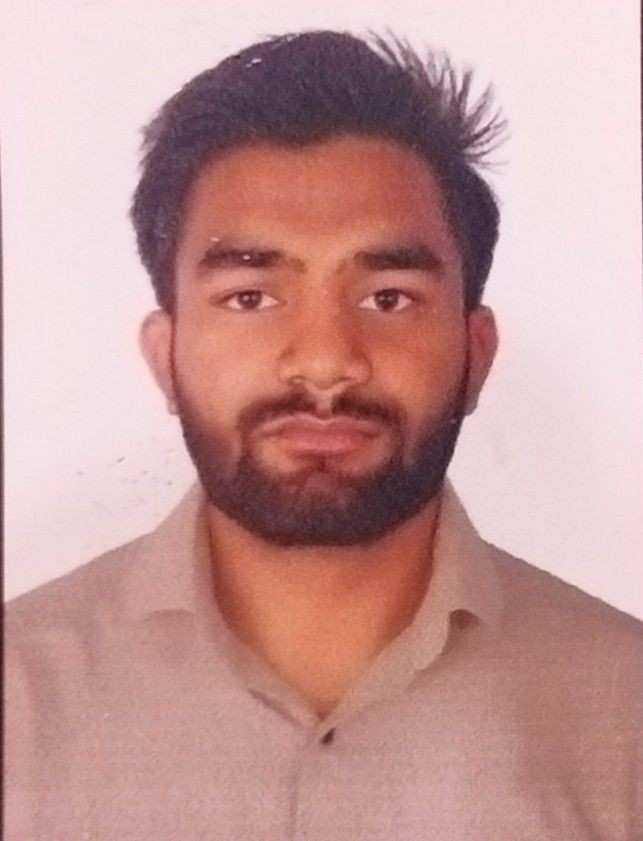
\includegraphics[width=2cm,clip]{me.png}

}\parbox{\dimexpr\linewidth-2.8cm\relax}{
\begin{tabularx}{\linewidth}{L r}
  \textbf{\LARGE \name} & +91-\phone\\
  {Roll No.:\roll} & \href{mailto:\emaila}{\emaila} \\
  \course &  \href{mailto:\emailb}{\emailb}\\
  {Electrical Engineering} &  \href{https://github.com/\github}{Github}  {}\\
  {EE Gate Qualified 2024} & \href{https://www.linkedin.com/in/\linkedin/}{linkedin.com/in/\linkedin}
\end{tabularx}
}



%-----------EDUCATION-----------------
% \section{Education}
%   \resumeSubHeadingListStart
%     \resumeSubheading
%       {Indian Institute of Technology Guwahati}{Guwahati, India}
%       {Bachelor of Technology in Mathematics and Computing ;  GPA: 8.10}{July. 2015 -- July. 2019 (Expected)}
%     \resumeSubheading
%       {Burdwan Model School}{Burdwan, W.B}
%       {Central Board of Secondary Education (Class XII);  Percentage: 96.60}{March. 2015}
%   \resumeSubHeadingListEnd\vspace{-3mm}
\section{\textcolor{headingColor}{\textbf{Education}}}
\setlength{\tabcolsep}{5pt} % Default value: 6pt
% \renewcommand{\arraystretch}{1.1} % Default value: 1https://www.overleaf.com/project/61fc166d7eab8975b2ab74d0
\small{\begin{tabularx}
{\dimexpr\textwidth-3mm\relax}{|c|C|c|c|}
  \hline
  \textbf{Degree/Certificate } & \textbf{Institute/Board} & \textbf{CGPA/Percentage} & \textbf{Year}\\
  \hline
  B.Tech Hons.(EE) & Rajkiya Engineering College, Mainpuri & 8.34 & 2023\\
  \hline
  %%Intermediate & Institute of Engineering and %%Management, Kolkata & 8.21 & 2015-2019\\ %Optional
 %% \hline
  Intermediate & U.P. Board & 73.8\% & 2018 \\
  \hline
  High School & U.P. Board & 80.67\% & 2016 \\
  \hline
\end{tabularx}}
\vspace{-2mm}

%-----------EXPERIENCE-----------------
\section{\textcolor{headingColor}{\textbf{Entrepreneurial Experience}}}
  \resumeSubHeadingListStart

    \resumeSubheading
      {Presence Learning Private Limited}{Mainpuri}
      {Founder | Presence Learning Private Limited}{Sept 2022 - Feb 2024}
      \resumeItemListStart
    \item {\textbf{Product Development}: Conceived and launched \textbf{"Mentor Series"}, a cutting-edge smart exam guide platform featuring QR codes for instant access to video solutions.}
    \item {\textbf{Team Leadership}: Recruited and managed a team of 25+ interns, organizing content creation, video production, editing, and overall workflow.}
    \item {\textbf{Technology Developement}: Developed a mobile app and website for book access and online delivery, achieving \textbf{1000+ app downloads}.}
   \item {\textbf{Operations Management}: Oversaw the creation and distribution of comprehensive smart books for 10+ subjects, producing 1000+ video lectures and establishing a robust dealer network across 15+ cities.}
   \item {\textbf{Sales and Marketing:}: Conducted webinars and social media marketing campaigns, resulting in the \textbf{sale of 1500+ books}.}
    \resumeItemListEnd
    
   %% \resumeSubheading
   %%   {Thinking Stack Inc.}{Bengaluru, India}
    %%  {Full Stack Developer Intern}{Dec. 2018 - Jan. %%2019}
   %%   \resumeItemListStart
   %% \item {Developed web app using ReactJS and deployed the app to AWS EC2 using Docker.}
  %%      \item {Made website mobile-friendly and increased Google web dev score by 50 points.}
  %%  \resumeItemListEnd
      
  \resumeSubHeadingListEnd
\vspace{-5.5mm}
%-----------PROJECTS-----------------
\section{\textcolor{headingColor}{\textbf{Projects}}}
\resumeSubHeadingListStart

    \resumeProject
      {Soil and Crop Analysis Using AI} %Project Name
      {Developed an advanced soil and crop analysis system utilizing machine learning to optimize agricultural productivity} %Project Name, Location Name
      {April. 2024} %Event Dates

      \resumeItemListStart
       \item {Designed and integrated a data collection system using Raspberry Pi and various soil sensors (e.g., moisture, pH, temperature).}
        \item {Developed a recommendation system for fertilizers and pesticides based on analysis results.}
        \item {Implemented machine learning algorithms to analyze soil data and predict crop health.}
        \item {\textbf{Tools \& technologies used}: Raspberry Pi, Sensors, Python, NodeJs, Html, CSS, Js}
    \resumeItemListEnd
    
    \resumeProject
      {Home Automation System Using website } %Project Name
      {Created a home automation system using Arduino, WiFi modules, and relays. } %Project Name, Location Name
      {Oct. 2022 - Dec. 2022} %Event Dates
    %  {\href{https://what-to-watch-next.herokuapp.com/}{Live Url} 
        %  |  {\href{https://github.com/ankit0696/what-to-watch-next}{Github}} } %Website

     \resumeItemListStart
       \item {Developed a web-based interface for remote control and monitoring of home devices.}
       \item {\textbf{Tools \& technologies used}: Arduino, Relay, PHP, Html, CSS, Js}
    \resumeItemListEnd
    
    \resumeProject
      {Smart Board for Touch and Laser Switch Control } %Project Name
      {Developed a smart board using MOSFETs and BC547 transistors for touch and laser switch control. } %Project Name, Location Name
      {Aug. 2021 - Sept. 2021} %Event Dates
     % {\href{https://github.com/ankit0696/kisan_mitra}%%{Github}} %Website
     
      \resumeItemListStart
         \item {\textbf{Tools \& technologies used}: Arduino, BC547 Transistor, LDR, Resistances, Relay, Diode}
    \resumeItemListEnd
    
     \resumeProject
      {Square Wave Inverter Design } %Project Name
      {Designed a square wave inverter using MOSFETs, diodes, 555 time IC and Relay. } %Project Name, Location Name
      {Nov. 2021 - Dec. 2021} %Event Dates
      %{\href{https://what-to-watch-next.herokuapp.com/}%{Live Url} 
        %  |  {\href{https://github.com/ankit0696/what-to-watch-next}{Github}} } %Website

     \resumeItemListStart
       \item {Conducted load testing to ensure reliable and efficient inverter operation.}
       \item {\textbf{Tools \& technologies used}: Transformer 220/12 V, Relay, Mosfet, Diode}
    \resumeItemListEnd 

      
          \resumeProject
      {Automatic Water Pump Control System } %Project Name
      {Designed a water pump control system using 555 timer IC, BC547 transistors, and relays. } %Project Name, Location Name
      {Nov. 2020 - Dec. 2020} %Event Dates
    %  {\href{https://what-to-watch-next.herokuapp.com/}{Live Url} 
         % |  {\href{https://github.com/ankit0696/what-to-watch-next}{Github}} } %Website

     \resumeItemListStart
       \item {Developed the circuit for automatic pump activation based on water levels.}
       \item {\textbf{Tools \& technologies used}:  Relay, Diode, Battery, BC547, 555 Timer IC, Resistors}
    \resumeItemListEnd 

          \resumeProject
      {WhatsApp Chatbot Platform for Customer Support and Sales } %Project Name
      {Developed a WhatsApp-based chatbot using NLP for customer support and sales. } %Project Name, Location Name
      {Dec. 2021 - Feb. 2022} %Event Dates
      %%{\href{https://what-to-watch-next.herokuapp.com/}{Live Url} 
        %%  |  {\href{https://github.com/ankit0696/what-to-watch-next}{Github}} } %Website

     \resumeItemListStart
       \item {Ensured scalability and reliability of the platform for handling large volumes of queries.}
       \item {\textbf{Tools \& technologies used}:  WhatsApp Business API, Python, Node Js, Database(Mysql), Reactjs, Rest APIs }
    \resumeItemListEnd 

          \resumeProject
      {Advanced CRM with AI for Sales Prediction and Lead Management } %Project Name
      {Designed and deployed a cloud-based CRM system enhanced with AI capabilities. } %Project Name, Location Name
      {March 2024.  - June. 2024} %Event Dates
     %% {\href{https://what-to-watch-next.herokuapp.com/}{Live Url} 
         %% |  {\href{https://github.com/ankit0696/what-to-watch-next}{Github}} } %Website

     \resumeItemListStart
       \item {Developed lead management features for tracking and prioritizing leads through the sales funnel.}
       \item {DIntegrated AI-driven analytics for generating actionable insights and recommendations.}
       \item {\textbf{Tools \& technologies used}:  TensorFlow, scikit-learn,  Python, Node Js, Database(Mysql), Reactjs, Rest APIs}
    \resumeItemListEnd 

          \resumeProject
      {Dynamic Certificate Generator for Interns } %Project Name
      {Developed a dynamic certificate generation system to create personalized certificates for interns.} %Project Name, Location Name
      {Dec. 2022 - Jan. 2023} %Event Dates
    %%  {\href{https://what-to-watch-next.herokuapp.com/}{Live Url} 
         %% |  {\href{https://github.com/ankit0696/what-to-watch-next}{Github}} } %Website

     \resumeItemListStart
      
       \item {\textbf{Tools \& technologies used}:  HTML/CSS, PHP, PDF Generation Libraries, SMTP}
    \resumeItemListEnd 
  \resumeSubHeadingListEnd
\vspace{-5.5mm}

%\section{Key Courses Taken}
%% \resumeHeadingSkillStart
%%  \resumeSubItem{} % Category
 %%   {Data Structure,Algorithms,DBMS,Machine Learning, Artificial Intelligence, Web Services, Operating System}
%  \resumeSubItem{Operating Systems}
%  {Windows, Linux*} 
% \hfill \textit{\footnotesize{* Elementary proficiency}} \hspace{3mm}
%% \resumeHeadingSkillEnd

\section{\textcolor{headingColor}{\textbf{Skills}}}
 \resumeHeadingSkillStart
 \resumeSubItem{Core Skills: } % Category
    { Circuit Design and Analysis,Embedded Systems (Python, Raspeberry Pi),Power Systems,Control Systems,Machines, Analog Electronics}
  \resumeSubItem{Programming: } % Category
    { C,Python,Nodejs, PHP, SQL}
 \resumeSubItem{Tools \& OS: } % Category
    {Arduino, Raspberry Pi, Motors, Transformers, Git, Linux, Windows } % Skills
 \resumeSubItem{Libraries/Frameworks: } % Category
    {Pandas, Numpy, scikit-learn, JQuery, Laravel}
    
     \resumeSubItem{Web Skills: } % Category
    {HTML/CSS/JS, Bootstrap, Wordpress}
    \resumeSubItem{Marketing Skills: } % Category
    {WhatsApp Marketing, Social Media Marketing, Indirect Marketing, Lead Generation}
%  \resumeSubItem{Operating Systems}
%  {Windows, Linux*} 
% \hfill \textit{\footnotesize{* Elementary proficiency}} \hspace{3mm}
 \resumeHeadingSkillEnd


\section{\textcolor{headingColor}{\textbf{Positions of Responsibility}}}
\vspace{-0.4mm}
\resumeSubHeadingListStart
\resumePOR{Director,} % Position
    {Presence Learning Private Limited} %Club,Event
    {Sept 2022 - Feb. 2024} %Tenure Period
\resumePOR{Team Cordinator, During Internship} % Position
    { 765/400 Kv Substation Mainpuri} %Club,Event
    {June. 2023 - July. 2023} %Tenure Period
\resumeSubHeadingListEnd
\vspace{-4mm}


\section{\textcolor{headingColor}{\textbf{Achievements}}}
\vspace{-0.4mm}
\resumeSubHeadingListStart
\resumePOR{Second Runner Up } % Award
    {Fake Investor, Technex, IIT BHU Won Prize of 1200/- } % Event
    {2023} %Event Year
    
%%\resumePOR{Winner } % Award
  %%  {Web Designing Competition(URECKON'18) organized by
  %%  
  %%  University of Engineering \\ \& Management, ISRO} % Event
  %%  {2018} %Event Year
    
  %%  \resumePOR{Github Arctic Code Vault Contributor } % Award
  %%  {Contributed code to several repositories in the 2020 GitHub \\ Archive Program} % Event
  %%  {2020} %Event Year

\resumeSubHeadingListEnd
\vspace{-4mm}

\section{\textcolor{headingColor}{\textbf{Certifications}}}
\vspace{-0.2mm}
\resumeSubHeadingListStart
\resumePOR{}{
NPTEL Certification on Patent Law for Engineers
}{Oct. 2022}

\resumePOR{}{
NPTEL Certification on Introduction to Industry 4.0 and Industrial Internet of Things
}{April 2021}
\resumePOR{}{
Coursera Certification on Excel Skills for Business
}{Sept. 2020}
\resumePOR{}{
Internshala Certification on Python
}{July 2020}
\resumeSubHeadingListEnd



\hspace*{-5mm}\rule{1.035\textwidth}{0.1mm}

%-------------------------------------------
\end{document}
